\documentclass[11pt]{standalone}


\usepackage{amssymb} 
\usepackage{amsmath} 

\usepackage[no-math]{fontspec}
\usepackage{unicode-math}
\setmainfont{Lato}
\setmathfont{Stix Two Math}

\usepackage{tikz}
\usetikzlibrary{arrows.meta}


\begin{document}
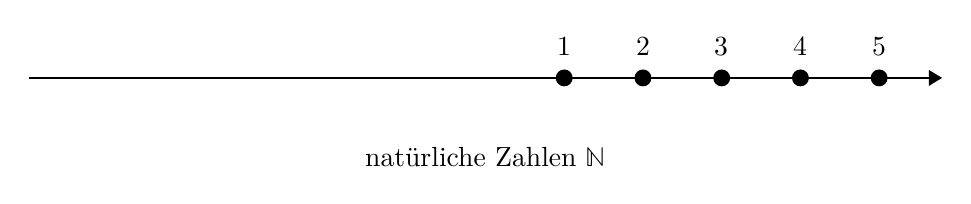
\begin{tikzpicture}
	\draw (0, -1) node {natürliche Zahlen $\mathbb{N}$};
	\draw [-{Triangle}, thick] (-5.8,0) -- (5.8,0);
	\foreach \x in {1,...,5} {
        \draw [fill] (\x,0) circle (0.1);
        \draw (\x,0.4) node {$\x$};
    }
\end{tikzpicture}
\end{document}